\chapter{Case Study}
\label{chap:case_study}

\section{Overview}

The goal of this chapter is to present a case study of a hierarchical runtime verification technology based on the previous chapters. The motive of this study is the related report from 2014 \citep{tdk2014}, which goal was a distributed, model based security logic. Their case study called the \emph{Model Railway Project}, and our study integrates their work, and finds ways to integrate it with other sensor sources for a hierarchical, more reliable security logic.

Because of this close relation to this railroad project, our focus will stay on railroad technologies and standards, it's important to notice our solution is a general approach for any critical system. This approach is based on controllability, observability, and hierarchy to increase a system general reliability, even when some of it's components are failing.

\begin{minipage}{\textwidth}
	\centering
	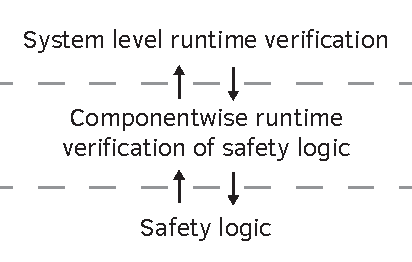
\includegraphics[width=0.75\linewidth]{include/figures/chapter_6/overview_1}
\end{minipage}

\section{Architecture}
	\subsection{Total view}
	Itt átvesszük a hardware alapjait, hogy egyáltalán miről van szó, hogy néz ki, mit tud.
	\subsection{Hardware}
	Itt az arduino alapú vezérlést emelném ki röviden, az ezzel felmerült problémákat, illetve a jövőbeli fejlesztések rövid bemutatását.

\section{Concept}
	A koncepció magyarázata, szép összefoglaló ábrával, és annak az összefoglalása, hogy mit tudunk ezzel elérni.

\section{Computer vision as a source of information}

\subsection{Hardware}

In case of a CV based approach, it is critical to choose the appropriate hardware. We had two parameters in the selection of the camera: height above the board, and FOV\footnote{Field of View}. 

These parameters are coupled, the heigher the camera, the less FOV we need. Most of the cameras on the market have FOV values approximately 60

\subsection{Introducing to OpenCV}

Az opencv rövid bemutatása, célja.

\subsection{Software}
\subsubsection{Mathematical solution}
A matematikai alap bemutatása, itt főleg a frekvenciatartomány beli mintakeresést kiemelve.
\subsubsection{CPU}
Az első implementáció gyors bemutatása.
\subsubsection{CUDA}
A GPU által gyorsított verzió bemutatása, mit tapasztaltunk ennek során, hogyan segített a fejlesztésben.

\section{Physical - Logical mapping}
	\subsection{Elements of logical mapping}
		Azoknak az elemeknek, elképzeléseknek az áttekintése, amik szerepelhetnek a modellünkben, még teljesen független módon.
	\subsection{Introducing to EMF}
		Az EMF bemutatása röviden.
	\subsection{Building the EMF model}
		Az elkészült EMF metamodell bemutatása, és összevetése az elképzelésekkel.
	\subsection{Introducing the IncQuery}
		Az IncQuery bemutatása.
	\subsection{Building the IncQuery patterns}
		A biztonsági lokikai patternek bemutatása.